\documentclass[a4paper,adobefonts,11pt,UTF8]{book}

%type chinese characters
\usepackage{ctex}

%Bibliography
\usepackage{chapterbib}
\usepackage[sectionbib,square,super,sort&compress]{natbib}


%generate index of book
\usepackage{makeidx}

\graphicspath{{../img/}}

%modify the headheight at least 13.5pt
\usepackage[headheight=13.6pt]{geometry}

%
\usepackage{fontspec}

%unicode
\usepackage{xunicode}

%
\usepackage{xltxtra}

%mathematics package
\usepackage{amsmath}

%mathematics symbols
\usepackage{amssymb}

%origin print package
\usepackage{verbatim}

%draw graphics use tikz and so on.
\usepackage{graphicx}

%set graphics path which used in the book.
\graphicspath{{../img/}}

%colorful table
\usepackage{colortbl}

%set color use origin name directly.
\usepackage[svgnames,table]{xcolor}

%
\usepackage[figuresright]{rotating}

% generate longtable which could across pages.
\usepackage{longtable}

%
\usepackage{multirow}

%
\usepackage{adjustbox}


%
\newcommand\mgape[1]{\gape{$\vcenter{\hbox{#1}}$}}

%
\usepackage{array}

%
\usepackage{makecell}

%
\usepackage{ulem}

%
\usepackage{color}

% draw graphics use tikz package
\usepackage{tikz}

%
\usepackage{listings}
\lstset{
  basicstyle=\ttfamily,
  showstringspaces=false,
  commentstyle=\color{red},
  keywordstyle=\color{blue},
  columns=flexible,
  backgroundcolor=\color{lightgray},
  extendedchars=true,
  basicstyle=\footnotesize\ttfamily,
  showstringspaces=false,
  showspaces=false,
  numbers=left,
  numberstyle=\footnotesize,
  numbersep=9pt,
  tabsize=2,
  breaklines=true,
  showtabs=false,
  captionpos=b
}

%
\usepackage{bashful}

%set book information including bookmarksnumbered,pdfencoding,
%pdfauthor,pdfpagelayout,breaklinks,colorlinks,linkcolor,
%urlcolor,and so on.
\usepackage[bookmarksnumbered,pdfencoding=auto,pdfauthor={穷屌丝联盟},pdfpagelayout=TwoPageRight,breaklinks,colorlinks,linkcolor=RoyalBlue,urlcolor=blue,colorlinks=true]{hyperref}

%add more list types.
\usepackage{paralist}

%set page styles
\usepackage{fancyhdr}

\pagestyle{fancy}
\fancyhf{}
\fancyhead[LE,RO]{\thepage}
\fancyhead[RE]{\leftmark}
\fancyhead[RO]{\rightmark}
\fancypagestyle{plain}{
  \fancyhf{}
  \renewcommand{\headrulewidth}{0pt}
}


%titlepage \titleGM
\newcommand*{\plogo}{\fbox{$\mathcal{PL}$}} % Generic publisher logo
%--------------------------------------------------------------------
% TITLE PAGE
%--------------------------------------------------------------------

\newcommand*{\titleGM}{\begingroup % Create the command for including the title page in the document
\hbox{ % Horizontal box
\hspace*{0.2\textwidth} % Whitespace to the left of the title page
\rule{1pt}{\textheight} % Vertical line
\hspace*{0.05\textwidth} % Whitespace between the vertical line and title page text
\parbox[b]{0.75\textwidth}{ % Paragraph box which restricts text to less than the width of the page
{\noindent\Huge\bfseries Notes Collection of \\[0.5\baselineskip] Regular Expression}\\[2\baselineskip] % Title
{\large \textit{Regular Expression}}\\[4\baselineskip] % Tagline or further description
{\Large \textsc{theqiong.com}} % Author name

\vspace{0.5\textheight} % Whitespace between the title block and the publisher
{\noindent 穷屌丝联盟}\\[\baselineskip] % Publisher and logo
}}
\endgroup}
%


%lstlisting[language=JavsScript]
% Taken from Lena Herrmann at 
% http://lenaherrmann.net/2010/05/20/javascript-syntax-highlighting-in-the-latex-listings-package
\definecolor{lightgray}{rgb}{.9,.9,.9}
\definecolor{darkgray}{rgb}{.4,.4,.4}
\definecolor{purple}{rgb}{0.65,0.12,0.82}

%lstlisting package -----------
% JavaScript
%------------------------------
\lstdefinelanguage{JavaScript}
{
  keywords={typeof,new,ture,false,catch,function,return,null,switch,var,if,in,while,do,else,case,break},
  keywordstyle=\color{blue}\bfseries,
  ndkeywords={class,export,boolean,throw,implements,import,this},
  ndkeywordstyle=\color{darkgray}\bfseries,
  identifierstyle=\color{black},
  sensitive=false,
  comment=[l]{//},
  morecomments[s]{/*}{*/},
  commentstyle=\color{purple}\ttfamily,
  stringstyle=\color{red}\ttfamily,
  morestring=[b]',
  morestring=[b]"
}

\lstdefinelanguage{Scheme}
{morekeywords={,lambda, cond, case, display, let, import, quote, quasiquote, unquote,
define, begin, newline, if, list, apply, null?, car, cdr, or, not, and, for-each, 
make-vector, vector-length, vector-ref, vector-set!, eqv?, eq?, equal?, else, set!, 
define-record-type, fields, mutable, immutable, assert, parent, with-exception-handler, }
sensitive=false,
morecomment=[l]{;},
morecomment=[s]{/*}{*/},
morestring=[b]",
}

\lstdefinelanguage{CSS}{
  morekeywords={accelerator,azimuth,background,background-attachment,
    background-color,background-image,background-position,
    background-position-x,background-position-y,background-repeat,
    behavior,border,border-bottom,border-bottom-color,
    border-bottom-style,border-bottom-width,border-collapse,
    border-color,border-left,border-left-color,border-left-style,
    border-left-width,border-right,border-right-color,
    border-right-style,border-right-width,border-spacing,
    border-style,border-top,border-top-color,border-top-style,
    border-top-width,border-width,bottom,caption-side,clear,
    clip,color,content,counter-increment,counter-reset,cue,
    cue-after,cue-before,cursor,direction,display,elevation,
    empty-cells,filter,float,font,font-family,font-size,
    font-size-adjust,font-stretch,font-style,font-variant,
    font-weight,height,ime-mode,include-source,
    layer-background-color,layer-background-image,layout-flow,
    layout-grid,layout-grid-char,layout-grid-char-spacing,
    layout-grid-line,layout-grid-mode,layout-grid-type,left,
    letter-spacing,line-break,line-height,list-style,
    list-style-image,list-style-position,list-style-type,margin,
    margin-bottom,margin-left,margin-right,margin-top,
    marker-offset,marks,max-height,max-width,min-height,
    min-width,-moz-binding,-moz-border-radius,
    -moz-border-radius-topleft,-moz-border-radius-topright,
    -moz-border-radius-bottomright,-moz-border-radius-bottomleft,
    -moz-border-top-colors,-moz-border-right-colors,
    -moz-border-bottom-colors,-moz-border-left-colors,-moz-opacity,
    -moz-outline,-moz-outline-color,-moz-outline-style,
    -moz-outline-width,-moz-user-focus,-moz-user-input,
    -moz-user-modify,-moz-user-select,orphans,outline,
    outline-color,outline-style,outline-width,overflow,
    overflow-X,overflow-Y,padding,padding-bottom,padding-left,
    padding-right,padding-top,page,page-break-after,
    page-break-before,page-break-inside,pause,pause-after,
    pause-before,pitch,pitch-range,play-during,position,quotes,
    -replace,richness,right,ruby-align,ruby-overhang,
    ruby-position,-set-link-source,size,speak,speak-header,
    speak-numeral,speak-punctuation,speech-rate,stress,
    scrollbar-arrow-color,scrollbar-base-color,
    scrollbar-dark-shadow-color,scrollbar-face-color,
    scrollbar-highlight-color,scrollbar-shadow-color,
    scrollbar-3d-light-color,scrollbar-track-color,table-layout,
    text-align,text-align-last,text-decoration,text-indent,
    text-justify,text-overflow,text-shadow,text-transform,
    text-autospace,text-kashida-space,text-underline-position,top,
    unicode-bidi,-use-link-source,vertical-align,visibility,
    voice-family,volume,white-space,widows,width,word-break,
    word-spacing,word-wrap,writing-mode,z-index,zoom},
  morestring=[s]{:}{;},
  sensitive,
  morecomment=[s]{/*}{*/}
}

\usepackage{pdfpages}


\renewcommand{\chaptername}{}
%%\titleformat{\chapter}[block]{\center\Huge}{\chaptername}{20pt}{}
%%\titleformat{\chapter}[block]{\center\Huge}{\chaptername}{20pt}{}
%%\makeatletter
\renewcommand{\bibname}{来源}



\setmainfont[Mapping=tex-text]{Minion Pro}

\makeindex


\title{{\zihao{1}Regular Expression Notes}}
\author{{\zihao{3}穷屌丝联盟}}
\date{\today}








\begin{document}

\begin{titlepage}
\addcontentsline{toc}{part}{Cover}

\pagestyle{empty} % Removes page numbers

\titleGM % This command includes the title page


\end{titlepage}

\maketitle
\tableofcontents
\listoffigures
\listoftables
\printindex

\part{Introduction}


正则表达式,又称正则表达式、正规表示法、常规表示法(英语:Regular Expression,在代码中常简写为regex、regexp或RE),计算机科学的一个概念。正则表达式使用单个字符串来描述、匹配一系列符合某个句法规则的字符串。在很多文本编辑器里,正则表达式通常被用来检索、替换那些符合某个模式的文本。

许多程序设计语言都支持利用正则表达式进行字符串操作。例如,在Perl中就内建了一个功能强大的正则表达式引擎。正则表达式这个概念最初是由Unix中的工具软件(例如sed和grep)普及开的。正则表达式通常缩写成“regex”,单数有regexp、regex,复数有regexps、regexes、regexen。

Regular Expression的“Regular”一般被译为“正则”、“正规”、“常规”。此处的“Regular”即是“规则”、“规律”的意思,Regular Expression即“描述某种规则的表达式”之意。

In computing, a regular expression (abbreviated regex or regexp)\cite{regular_expression} is a sequence of characters that forms a search pattern, mainly for use in pattern matching with strings, or string matching, i.e. ``find and replace"-like operations. The concept arose in the 1950s, when the American mathematician Stephen Kleene formalized the description of a regular language, and came into common use with the Unix text processing utilities ed, an editor, and grep (global regular expression print), a filter.

Each character in a regular expression is either understood to be a metacharacter with its special meaning, or a regular character with its literal meaning. Together, they can be used to identify textual material of a given pattern, or process a number of instances of it that can vary from a precise equality to a very general similarity of the pattern. The pattern sequence itself is an expression that is a statement in a language designed specifically to represent prescribed targets in the most concise and flexible way to direct the automation of text processing of general text files, specific textual forms, or of random input strings.

A very simple use of a regular expression would be to locate the same word spelled two different ways in a text editor, for example \textcolor{Blue}{\texttt{seriali[sz]e}}. A wildcard match can also achieve this, but wildcard matches differ from regular expressions in that wildcards are limited to what they can pattern (having fewer metacharacters and a simple language-base), whereas regular expressions are not. A usual context of wildcard characters is in globbing similar names in a list of files, whereas regular expressions are usually employed in applications that pattern-match text strings in general. For example, the simple regexp \verb|^[ \t]+||\verb|[ \t]+$| matches excess whitespace at the beginning and end of a line. An advanced regexp used to match any numeral is \verb|^[+-]?(\d+\.?\d*|\verb|\.\d+)([eE][+-]?\d+)?$|.

Many applications and programming languages have their own implementation of regular expressions, often with slight and sometimes with significant differences from other implementations. When two applications use a different implementation of regular expressions, we say that they use different ``regular expression flavors".


A regular expression processor processes a regular expression statement expressed in terms of a grammar in a given formal language, and with that examines the target text string, parsing it to identify substrings that are members of its language, the regular expressions.

Regular expressions are so useful in computing that the various systems to specify regular expressions have evolved to provide both a basic and extended standard for the grammar and syntax; modern regular expressions heavily augment the standard. Regular expression processors are found in several search engines, search and replace dialogs of several word processors and text editors, and in the command lines of text processing utilities, such as sed and AWK.

Many programming languages provide regular expression capabilities, some built-in, for example Perl, Ruby, AWK, and Tcl, and others via a standard library, for example .NET languages, Java, Python and C++ (since C++11). Most other languages offer regular expressions via a library.


\begin{figure}[!ht]
\centering
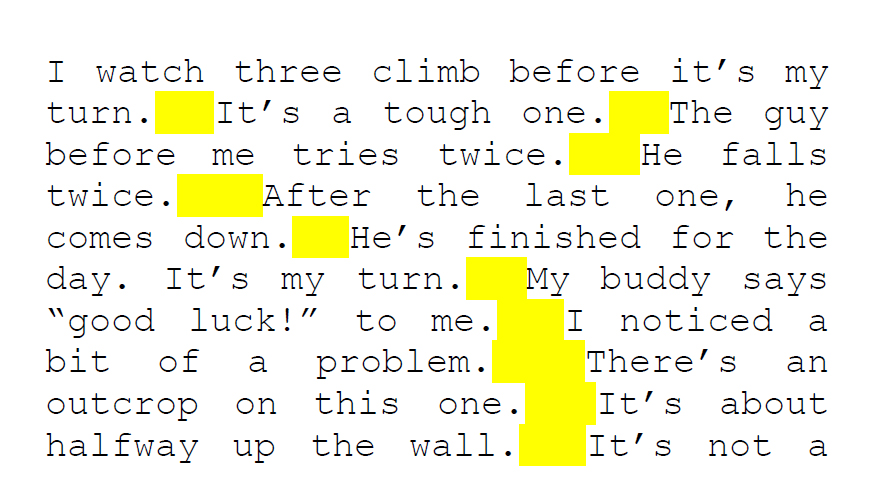
\includegraphics[scale=0.5]{The_river_effect_in_justified_text.jpg}
\vspace{-20pt}
\caption{\small{A regular expression like \textcolor{Blue}{\texttt{(?<=\textbackslash.) \{2,\}(?=[A-Z])}} would match the highlighted text above.}}
\label{regexp_example}
\end{figure}

注:上述正则表达式的意义如下:

\begin{compactenum}
\item \textcolor{Blue}{\texttt{(?<=\textbackslash.)}} 指定从每句话的结束符开始;
\item $\sqcup$\textcolor{Blue}{\texttt{\{2,\}}}指定只有具有多于两个空格时,才进行操作;
\item \textcolor{Blue}{\texttt{(?=[A-Z])}}指定空格至每一句的开头的大写字母为止。
\end{compactenum}



\chapter{History}


The origins of regular expressions lie in automata theory and formal language theory, both of which are part of theoretical computer science. These fields study models of computation (automata) and ways to describe and classify formal languages. In the 1950s, mathematician Stephen Cole Kleene described these models using his mathematical notation called \textsl{regular sets}. 

The SNOBOL language was an early implementation of pattern matching, but not identical to regular expressions. Among the first appearances of regular expressions in program form was when Ken Thompson built Kleene's notation into the editor QED as a means to match patterns in text files. He later added this capability to the Unix editor ed, which eventually led to the popular search tool grep's use of regular expressions (``grep" is a word derived from the command for regular expression searching in the ed editor: \texttt{g/re/p} meaning ``Global search for Regular Expression and Print matching lines"). Around the same time when Thompson developed QED, a group of researchers including Douglas T. Ross implemented a tool based on regular expressions that is used for lexical analysis in compiler design. Since that time, many variations of the original adaptations of regular expressions have been widely used in Unix and Unix-like utilities including expr, AWK, Emacs, vi, and lex.

Perl regular expressions derive from a regex library written by Henry Spencer, who later wrote an implementation of Advanced Regular Expressions for Tcl. The Tcl library is a hybrid NFA/DFA implementation with improved performance characteristics, earning praise from Jeffrey Friedl who said, ``...it really seems quite wonderful." Software projects that have adopted Spencer's Tcl regular expression implementation include PostgreSQL. Perl later expanded on Spencer's original library to add many new features, but has not yet caught up with Spencer's Advanced Regular Expressions implementation in terms of performance or Unicode handling. Philip Hazel developed PCRE (Perl Compatible Regular Expressions), which attempts to closely mimic Perl's regular expression functionality and is used by many modern tools including PHP and Apache HTTP Server. Part of the effort in the design of Perl 6 is to improve Perl's regular expression integration, and to increase their scope and capabilities to allow the definition of parsing expression grammars. The result is a mini-language called Perl 6 rules, which are used to define Perl 6 grammar as well as provide a tool to programmers in the language. These rules maintain existing features of Perl 5.x regular expressions, but also allow BNF-style definition of a recursive descent parser via sub-rules.

The use of regular expressions in structured information standards for document and database modeling started in the 1960s and expanded in the 1980s when industry standards like ISO SGML (precursored by ANSI ``GCA 101-1983") consolidated. The kernel of the structure specification language standards consists of regular expressions. Its use is evident in the DTD element group syntax.

最初的正则表达式出现于理论计算机科学的自动控制理论和形式化语言理论中。在这些领域中有对计算(自动控制)的模型和对形式化语言描述与分类的研究。 1940年,Warren McCulloch与Walter Pitts将神经系统中的神经元描述成小而简单的自动控制元。 1950年代,数学家斯蒂芬·科尔·克莱尼利用称之为“正则集合”的数学符号来描述此模型。肯·汤普逊将此符号系统引入编辑器QED,然后是Unix上的编辑器ed,并最终引入grep。自此,正则表达式被广泛地使用于各种Unix或者类似Unix的工具,例如Perl。

Perl的正则表达式源自于Henry Spencer写的regex,它已经演化成了pcre(Perl兼容正则表达式,Perl Compatible Regular Expressions),一个由Philip Hazel开发的,为很多现代工具所使用的库。

各计算机语言之间的正则表达式的集成目前开展的很差。未来的Perl6的子项目Apocalypse的设计中已考虑到了这点。




\chapter{Basic concepts}


A regular expression, often called a \textsf{pattern}, is an expression used to specify a set of strings required for a particular purpose. A simple way to specify a set of strings is simply to list its elements or members. However, there are often more concise ways to specify the desired set of strings. For example, the set containing the three strings ``Handel", ``Händel", and ``Haendel" can be specified by the \textsf{pattern} \textcolor{Blue}{\textsf{H(ä|ae?)ndel;}} we say that this pattern \textsf{matches} each of the three strings. In most formalisms, if there exists at least one regex that matches a particular set then there exists an infinite number of other regex that also match it—the specification is not unique. Most formalisms provide the following operations to construct regular expressions.

\begin{compactitem}
\item[1.~\textsf{Boolean ``or"}]  

A vertical bar(\textsf{|}) separates alternatives. For example, \textsf{pattern} \textcolor{Blue}{\textsf{gray|grey}} can match ``\textsf{gray}" or ``\textsf{grey}".

\item[2.~\textsf{Grouping}]

Parentheses are used to define the scope and precedence of the operators (among other uses). For example, \textsf{pattern} \textcolor{Blue}{\textsf{gray|grey}} and \textsf{pattern} \textcolor{Blue}{\textsf{gr(a|e)y}} are equivalent patterns which both describe the set of ``gray" or ``grey".

\item[3.~\textsf{Grouping}]

A quantifier after a token (such as a character) or group specifies how often that preceding element is allowed to occur. The most common quantifiers are the question mark \textsf{?}, the asterisk \textsf{*} (derived from the Kleene star), and the plus sign \textsf{+} (Kleene cross).

\begin{compactitem}
\item[\textsf{?}] The question mark indicates there is zero or one of the preceding element. For example, \textsf{colou?r} matches both ``\textsf{color}" and ``\textsf{colour}".
\item[\textsf{*}] The asterisk indicates there is zero or more of the preceding element. For example, \textsf{ab*c} matches ``\textsf{ac}", ``\textsf{abc}", ``\textsf{abbc}", ``\textsf{abbbc}", and so on.
\item[\textsf{+}] The plus sign indicates there is one or more of the preceding element. For example, \textsf{ab+c} matches ``\textsf{abc}", ``\textsf{abbc}", ``\textsf{abbbc}", and so on, but not ``\textsf{ac}".
\end{compactitem}

\end{compactitem}


These constructions can be combined to form arbitrarily complex expressions, much like one can construct arithmetical expressions from numbers and the operations +, −, ×, and ÷. For example, \textsf{H(ae?|ä)ndel} and \textsf{H(a|ae|ä)ndel} are both valid patterns which match the same strings as the earlier example, \textsf{H(ä|ae?)ndel}.

The precise syntax for regular expressions varies among tools and with context; more detail is given in the \hyperref[regular_expression_syntax]{Syntax section}.


正则表达式可以用形式化语言理论的方式来表达。正则表达式由常量和算子组成,它们分别指示字符串的集合和在这些集合上的运算。给定有限字母表Σ定义了下列常量:

\begin{compactitem}
\item (“空集”) $\emptyset$指示集合$\emptyset$∅
\item (“空串”) $\varepsilon$指示集合\{$\varepsilon$\}
\item (“文字字符”)在Σ中的a指示集合\{a\}
\end{compactitem}

定义了下列运算:


\begin{compactitem}
\item (“串接”) RS指示集合\{ αβ | α$\in$R,β$\in$S \}。例如:$$\text{\texttt{\{"ab","c"\}\{"d","ef"\} = \{"abd","abef","cd","cef"\}}}$$




\item (“选择”) R|S指示R和S的并集。例如:$$\text{\texttt{\{"ab","c"\}}|\texttt{\{"ab","d","ef"\}}}=\texttt{\{"ab","c","d","ef"\}}$$



\item (“Kleene星号”) R* 指示包含ε并且闭包在字符串串接下的R的最小超集。这是可以通过R中的零或多个字符串的串接得到所有字符串的集合。例如,$$\text{\texttt{\{"ab","c"\}* = \{}} \varepsilon \text{\texttt{,"ab","c","abab","abc","cab","cc","abaab","abcb",...\}}}$$



\end{compactitem}


上述常量和算子形成了克莱尼代数。很多课本使用对选择使用符号$\cup$, $+$或$\vee$替代竖杠。

为了避免括号,假定Kleene星号有最高优先级,接着是串接,接着是并集。如果没有歧义则可以省略括号。例如,\texttt{(ab)c}可以写为\texttt{abc}而\texttt{a|(b(c*))}可以写为\texttt{a|bc*}。

例子:

\begin{compactitem}
\item \texttt{a|b*}指示\texttt{\{$\varepsilon$,a,b,bb,bbb,...\}}。
\item \texttt{(a|b)*}指示由包括空串、任意数目个\texttt{a}或\texttt{b}字符组成的所有字符串的集合。
\item \texttt{ab*(c|$\varepsilon$)}指示开始于一个\texttt{a}接着零或多个\texttt{b}和最终可选的一个\texttt{c}的字符串的集合。
\end{compactitem}


正则表达式的定义非常精简,避免多余的量词\texttt{?}和\texttt{+},它们可以被表达为:\texttt{a+ = aa*}和\texttt{a? = (a|$\varepsilon$)}。

有时增加补算子~;~R指示在Σ* 上的不在R中的所有字符串的集合。补算子是多余的,因为它使用其他算子来表达(尽管计算这种表示的过程是复杂的,而结果可能以指数增大)。

这种意义上的正则表达式可以表达正则语言,精确的是可被有限状态自动机接受的语言类。但是在简洁性上有重要区别。某类正则语言只能用大小指数增长的自动机来描述,而要求的正则表达式的长度只线性的增长。

正则表达式对应于乔姆斯基层级的类型-3文法。在另一方面,在正则表达式和不导致这种大小上的爆炸的非确定有限状态自动机(NFA)之间有简单的映射,为此NFA经常被用作正则表达式的替代表示。

我们还要在这种形式化中研究表达力。如下面例子所展示的,不同的正则表达式可以表达同样的语言:这种形式化中存在着冗余。

有可能对两个给定正则表达式写一个算法来判定它们所描述的语言是否本质上相等,简约每个表达式到极小确定有限自动机,确定它们是否同构(等价)。

这种冗余可以消减到什么程度?我们可以找到仍有完全表达力的正则表达式的有趣的子集吗? Kleene星号和并集明显是需要的,但是我们或许可以限制它们的使用。这提出了一个令人惊奇的困难问题。因为正则表达式如此简单,没有办法在语法上把它重写成某种规范形式。过去公理化的缺乏导致了星号高度问题。最近Dexter Kozen用克莱尼代数公理化了正则表达式。

很多现实世界的“正则表达式”引擎实现了不能用正则表达式代数表达的特征。

\chapter{Formal language theory}

Regular expressions describe regular languages in formal language theory. They have the same expressive power as regular grammars.






\section{Formal definition}

Regular expressions consist of constants and operator symbols that denote sets of strings and operations over these sets, respectively. The following definition is standard, and found as such in most textbooks on formal language theory. Given a finite alphabet Σ, the following constants are defined as regular expressions:


\begin{compactitem}
\item (\textsf{empty set}) $\emptyset$ denoting the set $\emptyset$.
\item (\textsf{empty string}) $\varepsilon$ denoting the set containing only the ``empty" string, which has no characters at all.
\item (\textsf{literal character}) a in Σ denoting the set containing only the character a.
\end{compactitem}


Given regular expressions R and S, the following operations over them are defined to produce regular expressions:

\begin{compactitem}
\item (\textsf{concatenation}) RS denoting the set \{ αβ | α in set described by expression R and β in set described by S \}. For example $$\text{\texttt{\{"ab","c"\}\{"d","ef"\} = \{"abd","abef","cd","cef"\}}}$$
\item (\textsf{alternation}) R | S denoting the set union of sets described by R and S. For example, 

if R describes \texttt{\{"ab","c"\}} and S describes \texttt{\{"ab", "d", "ef"\}}, expression R | S describes \texttt{\{"ab", "c", "d", "ef"\}}.$$\text{\texttt{\{"ab","c"\}}|\texttt{\{"ab","d","ef"\}}}=\texttt{\{"ab","c","d","ef"\}}$$
\item (\textsf{Kleene star}) R* denoting the smallest superset of set described by R that contains ε and is closed under string concatenation. This is the set of all strings that can be made by concatenating any finite number (including zero) of strings from set described by R. For example, \texttt{\{"0","1"\}*} is the set of all finite binary strings (including the empty string), and 
$$\text{\texttt{\{"ab","c"\}* = \{}} \varepsilon \text{\texttt{,"ab","c","abab","abc","cab","cc","abaab","abcb",...\}}}$$
\end{compactitem}

To avoid parentheses it is assumed that the Kleene star has the highest priority, then concatenation and then alternation. If there is no ambiguity then parentheses may be omitted. For example, \texttt{(ab)c} can be written as \text{abc}, and \texttt{a|(b(c*))} can be written as \texttt{a|bc*}. Many textbooks use the symbols $\cup$, $+$, or $\vee$ for alternation instead of the vertical bar.

Examples:

\begin{compactitem}
\item \texttt{a|b*} denotes $$\text{\texttt{\{}} \varepsilon \text{\texttt{,"a","b","bb","bbb",...\}}}$$
\item \texttt{(a|b)*} denotes the set of all strings with no symbols other than ``\texttt{a}" and ``\texttt{b}", including the empty string: $$\text{\texttt{\{}} \varepsilon \text{\texttt{,"a","b","aa","ab","ba","bb","aaa",...\}}}$$
\item \texttt{ab*(c|ε)} denotes the set of strings starting with ``\texttt{a}", then zero or more ``\texttt{b}"s and finally optionally a ``\texttt{c}": $$\text{\texttt{\{"a","ac","ab","abc","abb","abbc",...\}}}$$

\end{compactitem}




\section{Expressive power and compactness}

The formal definition of regular expressions is purposely parsimonious and avoids defining the redundant quantifiers \texttt{?} and \texttt{+}, which can be expressed as follows: \texttt{a+ = aa*}, and \texttt{a? = (a|$\varepsilon$)}. Sometimes the complement operator is added, to give a generalized regular expression; here Rc matches all strings over \texttt{Σ*} that do not match R. In principle, the complement operator is redundant, as it can always be circumscribed by using the other operators. However, the process for computing such a representation is complex, and the result may require expressions of a size that is double exponentially larger.

Regular expressions in this sense can express the regular languages, exactly the class of languages accepted by deterministic finite automata. There is, however, a significant difference in compactness. Some classes of regular languages can only be described by deterministic finite automata whose size grows exponentially in the size of the shortest equivalent regular expressions. The standard example here is the languages Lk consisting of all strings over the alphabet \texttt{\{a,b\}} whose kth-from-last letter equals a. On one hand, a regular expression describing L4 is given by $$\text{\texttt{|(a|b)\^{}*a(a|b)(a|b)(a|b)|}}$$


Generalizing this pattern to $L_k$ gives the expression$$(a|b)^*a\underbrace{(a|b)(a|b)\cdots(a|b)}_{k-1\text{  times}}$$

On the other hand, it is known that every deterministic finite automaton accepting the language Lk must have at least 2k states. Luckily, there is a simple mapping from regular expressions to the more general nondeterministic finite automata (NFAs) that does not lead to such a blowup in size; for this reason NFAs are often used as alternative representations of regular languages. NFAs are a simple variation of the type-3 grammars of the Chomsky hierarchy.

Finally, it is worth noting that many real-world ``regular expression" engines implement features that cannot be described by the regular expressions in the sense of formal language theory.




\section{Deciding equivalence of regular expressions}

As seen in many of the examples above, there is more than one way to construct a regular expression to achieve the same results.

It is possible to write an algorithm which for two given regular expressions decides whether the described languages are essentially equal, reduces each expression to a minimal deterministic finite state machine, and determines whether they are isomorphic (equivalent).

The redundancy can be eliminated by using Kleene star and set union to find an interesting subset of regular expressions that is still fully expressive, but perhaps their use can be restricted. This is a surprisingly difficult problem. As simple as the regular expressions are, there is no method to systematically rewrite them to some normal form. The lack of axiom in the past led to the star height problem. In 1991, Dexter Kozen axiomatized regular expressions with Kleene algebra.



\chapter{Syntax}
\label{regular_expression_syntax}

Any non-trivial regex looks daunting to anybody not familiar with them. But with just a bit of experience, you will soon be able to craft your own regular expressions like you have never done anything else. 

A regular expression (regex or regexp for short) is a special text string for describing a search pattern. You can think of regular expressions as wildcards on steroids. You are probably familiar with wildcard notations such as \colorbox{lightgray}{\texttt{*.txt}} to find all text files in a file manager. The regex equivalent is \colorbox{lightgray}{\texttt{.*\textbackslash .txt\$}}.\cite{regexp_wildcard}

But you can do much more with regular expressions, you could use the regular expression \colorbox{lightgray}{\texttt{\textbackslash b[A-Z0-9.\_\%+-]+@[A-Z0-9.-]+\textbackslash .[A-Z]\{2,4\}\textbackslash b}} to search for an email address. Any email address, to be exact. A very similar regular expression (replace the first \colorbox{lightgray}{\texttt{\textbackslash b}} with \colorbox{lightgray}{\texttt{\^{}}} and the last one with \colorbox{lightgray}{\texttt{\$}}) can be used by a programmer to check whether the user entered a properly formatted email address. In just one line of code, whether that code is written in Perl, PHP, Java, a .NET language, or a multitude of other languages.

A regexp pattern matches a target string. The pattern is composed of a sequence of atoms. An atom is what matches at a point in the target string. The simplest atom is a literal, but grouping parts of the pattern to match an atom will require using \texttt{( )} as metacharacters. Metacharacters help form: atoms; quantifiers telling how many atoms (and whether it is a greedy quantifier or not); a logical OR character, which offers a set of alternatives, and a logical NOT character, which negates an atom's existence; and back references to refer to previous atoms of a completing pattern of atoms. A match is made, not when all the atoms of the string are matched, but rather when all the pattern atoms in the regular expression have matched. The idea is to make a small pattern of characters stand for a large number of possible strings, rather than compiling a large list of all the literal possibilities.

Depending on the regexp processor there are about fourteen metacharacters, characters that may or may not have their literal character meaning, depending on context, or whether they are ``escaped", i.e., preceded by an escape sequence, in this case, the backslash \textbackslash. Modern and POSIX extended regular expressions use metacharacters more often than their literal meaning, so to avoid ``backslash-osis" it makes sense to have a metacharacter escape to a literal mode; but starting out, it makes more sense to have the four bracketing metacharacters \texttt{( )} and \texttt{\{ \}} be primarily literal, and ``escape" that usual meaning to become metacharacters. Common standards implement both. The usual metacharacters are \texttt{\{\}[]()\^{}\$.|*+?} and \textbackslash. The usual characters that become metacharacters when escaped are dsw.DSW and N.





\section{Delimiters}


When entering a regular expression in a programming language, they may be represented as a usual string literal, hence usually quoted; this is common in C, Java, and Python for instance, where the regular expression re is entered as ``re". However, they are often written with slashes as delimiters, as in \texttt{/re/} for the regular expression re. This originates in ed, where \texttt{/} is the editor command for searching, and an expression \texttt{/re/} can be used to specify a range of lines (matching the pattern), which can be combined with other commands on either side, most famously \texttt{g/re/p} as in grep (``global regex print"). A similar convention is used in sed, where search and replace is given by s/regexp/replacement/ and patterns can be joined with a comma to specify a range of lines as in \texttt{/re1/,/re2/}. This notation is particularly well-known due to its use in Perl, where it forms part of the syntax distinct from normal string literals. In some cases, such as sed and Perl, alternative delimiters can be used to avoid collision with contents, and to avoid having to escape the delimiters. For example, in sed the command \texttt{s,/,X,} will replace a \texttt{/} with an \texttt{X}, using commas as delimiters.



一个正则表达式通常被称为一个模式(pattern),为用来描述或者匹配一系列符合某个句法规则的字符串。例如:Handel、Händel和Haendel这三个字符串,都可以由“\texttt{Ha|ä|(ae)ndel}”这个模式来描述。大部分正则表达式的形式都有如下的结构:

\begin{compactitem}
\item \textbf{选择}

|竖直分隔符代表选择。例如“\texttt{gray|grey}”可以匹配\texttt{grey}或\texttt{gray}。

\item \textbf{数量限定}

某个字符后的数量限定符用来限定前面这个字符允许出现的个数。最常见的数量限定符包括“+”、“?”和“*”(不加数量限定则代表出现一次且仅出现一次):

\begin{compactitem}
\item \textbf{+}加号代表前面的字符必须至少出现一次。(1次、或多次)。例如,“\texttt{goo+gle}”可以匹配\texttt{google}、\texttt{gooogle}、\texttt{goooogle}等;
\item \textbf{?}问号代表前面的字符最多只可以出现一次。(0次、或1次)。例如,“colou?r”可以匹配color或者colour;
\item \textbf{*}星号代表前面的字符可以不出现,也可以出现一次或者多次。(0次、或1次、或多次)。例如,“\texttt{0*42}”可以匹配\texttt{4}2、\texttt{042}、\texttt{0042}、\texttt{00042}等。

\end{compactitem}

\item \textbf{匹配}

圆括号可以用来定义操作符的范围和优先度。例如,“\texttt{gr(a|e)y}”等价于“\texttt{gray|grey}”,“\texttt{(grand)?father}”匹配\texttt{father}和\texttt{grandfather}。




\end{compactitem}

上述这些构造子都可以自由组合,因此,“\texttt{H(ae?|ä)ndel}”和“\texttt{H(a|ae|ä)ndel}”是相同的。

精确的语法可能因不同的工具或程序而异。


\section{Standards}

The IEEE POSIX standard has three sets of compliance: BRE, ERE, and SRE for Basic, Extended, and Simple Regular Expressions. SRE is deprecated, in favor of BRE, as both provide backward compatibility. The subsection below covering the character classes applies to both BRE and ERE.

BRE and ERE work together. ERE adds \texttt{?, +,} and \texttt{|,} and it removes the need to escape the metacharacters \texttt{( )} and \texttt{\{ \}}, which are required in BRE. Furthermore, as long as the POSIX standard syntax for regular expressions is adhered to, there can be, and often is, additional syntax to serve specific (yet POSIX compliant) applications. Although POSIX.2 leaves some implementation specifics undefined, BRE and ERE provide a ``standard" which has since been adopted as the default syntax of many tools, where the choice of BRE or ERE modes is usually a supported option. For example, GNU grep has the following options: ``\texttt{grep -E}" for ERE, and "``\texttt{grep -G}" for BRE (the default), and ``\texttt{grep -P}" for Perl regular expressions.

Perl regular expressions have become a de facto standard, having a rich and powerful set of atomic expressions. Perl has no ``basic" "extended" level, where the \texttt{( )} and \texttt{\{ \}} may or may not have literal meanings. They are always metacharacters, as they are in ``extended" mode for POSIX. To get their literal meaning, you escape them. Other metacharacters are known to be literal or symbolic based on context alone. Perl offers much more functionality: ``lazy" regular expressions, backtracking, named capture groups, and recursive patterns, all of which are powerful additions to POSIX BRE/ERE.



\subsection{POSIX basic and extended}

In the POSIX standard, Basic Regular Syntax, BRE, requires that the metacharacters \texttt{( )} and \texttt{\{ \}} be designated \texttt{\textbackslash(\textbackslash)} and \texttt{\textbackslash\{\textbackslash\}}, whereas Extended Regular Syntax, ERE, does not.


\subsection{POSIX extended}




\subsection{Character classes}



\section{Standard Perl}




\section{Lazy quantification}







\chapter{Patterns for non-regular languages}






\chapter{Fuzzy regular expressions}







\chapter{Implementations and running times}





\chapter{Unicode}







\chapter{Uses}

A replacement string, also known as the replacement text, is the text that each regular expression match is replaced with during a search-and-replace. In most applications, the replacement text supports special syntax that allows you to reuse the text matched by the regular expression or parts thereof in the replacement. While replacement strings are fairly simple compared with regular expressions, there is still great variety between the syntax used by various applications and their actual behavior.

There are many software applications and programming languages that support regular expressions. If you are a programmer, you can save yourself lots of time and effort. You can often accomplish with a single regular expression in one or a few lines of code what would otherwise take dozens or hundreds.

If you are not a programmer, you can use regular expressions in many situations just as well. They make finding information a lot easier. You can use them in powerful search and replace operations to quickly make changes across large numbers of files. A simple example is \colorbox{lightgray}{\texttt{gr[ae]y}} which finds both spellings of the word gray in one operation, instead of two. There are many text editors and search and replace tools with decent regex support.







\chapter{Examples}




























































\bibliographystyle{plainnat}
\bibliography{REN}
\clearpage

\part{Foundation}

Many applications and programming languages have their own implementation of regular expressions, often with slight and sometimes with significant differences from other implementations. When two applications use a different implementation of regular expressions, we say that they use different ``regular expression flavors". 



%%====================================
%% 文本模式和匹配
%%====================================

\chapter{Text Patterns and Matches}



A regular expression, or regex for short, is a pattern describing a certain amount of text. This first example \colorbox{lightgray}{\texttt{regex}} is actually a perfectly valid regex. It is the most basic pattern, simply matching the literal text \colorbox{lightgray}{\texttt{regex}}.


















%%====================================
%% 文本字符
%%====================================

\chapter{Literal Characters}


The most basic regular expression consists of a single literal character, such as \colorbox{lightgray}{\texttt{a}}. It matches the first occurrence of that character in the string. If the string is \colorbox{lightgray}{\texttt{Jack is a boy}}, it matches the \colorbox{lightgray}{\texttt{a}} after the \colorbox{lightgray}{\texttt{J}}.


This regex can match the second \colorbox{lightgray}{\texttt{a}} too. It only does so when you tell the regex engine to start searching through the string after the first match. In a text editor, you can do so by using its \colorbox{lightgray}{\texttt{"Find Next"}} or \colorbox{lightgray}{\texttt{"Search Forward"}} function. In a programming language, there is usually a separate function that you can call to continue searching through the string after the previous match.

Twelve characters have special meanings in regular expressions: the backslash \colorbox{lightgray}{\texttt{\textbackslash}}, the caret \colorbox{lightgray}{\texttt{\^{}}}, the dollar sign \colorbox{lightgray}{\texttt{\$}}, the period or dot \colorbox{lightgray}{\texttt{.}}, the vertical bar or pipe symbol \colorbox{lightgray}{\texttt{|}}, the question mark \colorbox{lightgray}{\texttt{?}}, the asterisk or star \colorbox{lightgray}{\texttt{*}}, the plus sign \colorbox{lightgray}{\texttt{+}}, the opening parenthesis \colorbox{lightgray}{\texttt{(}}, the closing parenthesis \colorbox{lightgray}{\texttt{)}}, the opening square bracket \colorbox{lightgray}{\texttt{[}}, and the opening curly brace \colorbox{lightgray}{\texttt{\{}}. These special characters are often called "metacharacters".


If you want to use any of these characters as a literal in a regex, you need to escape them with a backslash. If you want to match \colorbox{lightgray}{\texttt{1+1=2}}, the correct regex is \colorbox{lightgray}{\texttt{1\textbackslash +1=2}}. Otherwise, the plus sign has a special meaning.




%%====================================
%% 字符类或字符集
%%====================================

\chapter{Character Classes or Character Sets}

A ``character class" matches only one out of several characters. To match an \texttt{a} or an \texttt{e}, use \colorbox{lightgray}{\texttt{[ae]}}. You could use this in \colorbox{lightgray}{\texttt{gr[ae]y}} to match either \texttt{gray} or \texttt{grey}. A character class matches only a single character. \colorbox{lightgray}{\texttt{gr[ae]y}} does not match \texttt{graay}, \texttt{graey} or any such thing. The order of the characters inside a character class does not matter.


You can use a hyphen inside a character class to specify a range of characters. \colorbox{lightgray}{\texttt{[0-9]}} matches a single digit between 0 and 9. You can use more than one range. \colorbox{lightgray}{\texttt{[0-9a-fA-F]}} matches a single hexadecimal digit, case insensitively. You can combine ranges and single characters. \colorbox{lightgray}{\texttt{[0-9a-fxA-FX]}} matches a hexadecimal digit or the letter \textsf{X}.


Typing a caret after the opening square bracket negates the character class. The result is that the character class matches any character that is not in the character class. \colorbox{lightgray}{\texttt{q[\^{}x]}} matches \colorbox{lightgray}{\texttt{qu}} in \texttt{question}. It does not match \colorbox{lightgray}{\texttt{Iraq}} since there is no character after the \textsf{q} for the negated character class to match.


%%====================================
%% 简写字符类
%%====================================

\chapter{Shorthand Character Classes}


\colorbox{lightgray}{\texttt{\textbackslash d}} matches a single character that is a digit, \colorbox{lightgray}{\texttt{\textbackslash w}} matches a ``word character" (alphanumeric characters plus underscore), and \colorbox{lightgray}{\texttt{\textbackslash s}} matches a whitespace character (includes tabs and line breaks). The actual characters matched by the shorthands depends on the software you're using. In modern applications, they include non-English letters and numbers.


%%====================================
%% 非打印字符类
%%====================================

\chapter{Non-Printable Characters}


You can use special character sequences to put non-printable characters in your regular expression. Use \colorbox{lightgray}{\texttt{\textbackslash t}} to match a tab character (ASCII 0x09), \colorbox{lightgray}{\texttt{\textbackslash r}} for carriage return (0x0D) and \colorbox{lightgray}{\texttt{\textbackslash n}} for line feed (0x0A). More exotic non-printables are \colorbox{lightgray}{\texttt{\textbackslash a}} (bell, 0x07), \colorbox{lightgray}{\texttt{\textbackslash e}} (escape, 0x1B), \colorbox{lightgray}{\texttt{\textbackslash f}} (form feed, 0x0C) and \colorbox{lightgray}{\texttt{\textbackslash v}} (vertical tab, 0x0B). Remember that Windows text files use \colorbox{lightgray}{\texttt{\textbackslash r\textbackslash n}} to terminate lines, while UNIX text files use \colorbox{lightgray}{\texttt{\textbackslash n}}.


If your application supports Unicode, use \colorbox{lightgray}{\texttt{\textbackslash uFFFF}} or \colorbox{lightgray}{\texttt{\textbackslash x\{FFFF\}}} to insert a Unicode character. \colorbox{lightgray}{\texttt{\textbackslash u20AC}} or \colorbox{lightgray}{\texttt{\textbackslash x\{20AC\}}} matches the euro currency sign.


If your application does not support Unicode, use \colorbox{lightgray}{\texttt{\textbackslash xFF}} to match a specific character by its hexadecimal index in the character set. \colorbox{lightgray}{\texttt{\textbackslash xA9}} matches the copyright symbol in the Latin-1 character set.

All non-printable characters can be used directly in the regular expression, or as part of a character class.


%%====================================
%% 点匹配字符
%%====================================

\chapter{Dot Matches}

The dot matches a single character, except line break characters. It is short for \colorbox{lightgray}{\texttt{[\^{}\textbackslash n]}} (UNIX applications) or \colorbox{lightgray}{\texttt{[\^{}\textbackslash r\textbackslash n]}} (Windows applications). Most applications have a ``dot matches all" or ``single line" mode that makes the dot match any single character, including line breaks.

\colorbox{lightgray}{\texttt{gr.y}} matches \texttt{gray}, \texttt{grey}, \texttt{gr\%y}, etc. Use the dot sparingly. Often, a character class or negated character class is faster and more precise.


%%====================================
%% 锚
%%====================================

\chapter{Anchors}


Anchors do not match any characters. They match a position. \colorbox{lightgray}{\texttt{\^{}}} matches at the start of the string, and \colorbox{lightgray}{\texttt{\$}} matches at the end of the string. Most regex engines have a "``multi-line" mode that makes \colorbox{lightgray}{\texttt{\^{}}} match after any line break, and \colorbox{lightgray}{\texttt{\$}} before any line break. E.g. \colorbox{lightgray}{\texttt{\^{}b}} matches only the first b in \texttt{bob}.


\colorbox{lightgray}{\texttt{\textbackslash b}} matches at a word boundary. A word boundary is a position between a character that can be matched by \colorbox{lightgray}{\texttt{\textbackslash w}} and a character that cannot be matched by \colorbox{lightgray}{\texttt{\textbackslash w}}. \colorbox{lightgray}{\texttt{\textbackslash b}} also matches at the start and/or end of the string if the first and/or last characters in the string are word characters. \colorbox{lightgray}{\texttt{\textbackslash B}} matches at every position where \colorbox{lightgray}{\texttt{\textbackslash b}} cannot match.




%%====================================
%% 轮换
%%====================================

\chapter{Alternation}


Alternation is the regular expression equivalent of ``or". \colorbox{lightgray}{\texttt{cat|dog}} matches \colorbox{lightgray}{\texttt{cat}} in \colorbox{lightgray}{\texttt{About cats and dogs}}. If the regex is applied again, it matches \colorbox{lightgray}{\texttt{dog}}. You can add as many alternatives as you want: \colorbox{lightgray}{\texttt{cat|dog|mouse|fish}}.

Alternation has the lowest precedence of all regex operators. \colorbox{lightgray}{\texttt{cat|dog food}} matches \colorbox{lightgray}{\texttt{cat}} or \colorbox{lightgray}{\texttt{dog food}}. To create a regex that matches cat food or dog food, you need to group the alternatives: \colorbox{lightgray}{\texttt{(cat|dog) food}}.


%%====================================
%% 重复
%%====================================

\chapter{Repetition}


The question mark makes the preceding token in the regular expression optional. \colorbox{lightgray}{\texttt{colou?r}} matches \texttt{colour} or \texttt{color}.


The asterisk or star tells the engine to attempt to match the preceding token zero or more times. The plus tells the engine to attempt to match the preceding token once or more. 

\colorbox{lightgray}{\texttt{<[A-Za-z][A-Za-z0-9]*>}} matches an HTML tag without any attributes. \colorbox{lightgray}{\texttt{<[A-Za-z0-9]+>}} is easier to write but matches invalid tags such as \texttt{<1>}.

Use curly braces to specify a specific amount of repetition. Use \colorbox{lightgray}{\texttt{\textbackslash b[1-9][0-9]\{3\}\textbackslash b}} to match a number between 1000 and 9999. \colorbox{lightgray}{\texttt{\textbackslash b[1-9][0-9]\{2,4\}\textbackslash b}} matches a number between 100 and 99999.





%%====================================
%% 贪婪和懒惰重复
%%====================================

\chapter{Greedy and Lazy Repetition}












%%====================================
%% 分组和捕获
%%====================================

\chapter{Grouping and Capturing}












%%====================================
%% 反向引用
%%====================================

\chapter{Backreferences}





%%====================================
%% 命名组和反向引用
%%====================================

\chapter{Named Groups and Backreferences}





%%====================================
%% Unicode
%%====================================

\chapter{Unicode Properties}








%%====================================
%% 环视
%%====================================

\chapter{Lookaround}









%%====================================
%% 自由间隔语法
%%====================================

\chapter{Free-Spacing Syntax}













\bibliographystyle{plainnat}
\bibliography{VEN}
\clearpage


\end{document}


























